% !TeX root = ./conference_071817.tex
\documentclass[conference]{IEEEtran}
\IEEEoverridecommandlockouts
% The preceding line is only needed to identify funding in the first footnote. If that is unneeded, please comment it out.
\usepackage{cite}
\usepackage{amsmath,amssymb,amsfonts}
\usepackage{algorithmic}
\usepackage{graphicx}
\usepackage{textcomp}
\usepackage{color}
\usepackage{ulem}
%\usepackage{natbib}


\newcommand{\MK}[1]{\textcolor{red}{MK: #1}}  % Manoj's comments

\def\BibTeX{{\rm B\kern-.05em{\sc i\kern-.025em b}\kern-.08em
    T\kern-.1667em\lower.7ex\hbox{E}\kern-.125emX}}
\begin{document}

\title{Evaluation and Analysis of Methods for Facial Recognition Applied to Partially Occluded Images}

\author{\IEEEauthorblockN{Zahra Siddiqa}
School of Computing\\
Dublin City University\\
Dublin, Ireland \\
\textit{zahara.hassan2@mail.dcu.ie
}}

\maketitle



\begin{abstract}
Face recognition algorithm provides capability to the systems to detect and identify human faces. Face recognition systems find applications in access and security, criminal identification, target advertising, computer vision and many other fields. It is easier to build a face recognition system when an image contains unobstructed view of the face. However in the real world, the probability of finding images with a partial or occluded face is very high which hinders the performance of the face recognition systems. The aim of this project is to understand if the existing machine learning methods can be used for face recognition under occluded conditions without compromising on the accuracy. To achieve this, a comparative analysis in the form of an experiment has been performed on existing methods of face recognition applied to occluded images. As a result, this project confirms the higher degree of accuracy that can be achieved with convolutional neural networks over other methods.
\end{abstract}

\begin{IEEEkeywords}
Face Recognition; Occlusion; Principal Component Analysis; K Nearest Neighbour; Convolutional Neural Networks;

\end{IEEEkeywords}

\section{Introduction}
\label{sec: 1.introduction}

Unlike face detection which deals with identifying the presence of a face in an image, face recognition deals with the feature extraction and recognition of the face in an image. Facial recognition techniques have proven beneficial predominantly in the field of security. Face recognition is the preferred choice over other biometrics like iris scans or fingerprints as it is a non intrusive and robust method of identification. As a whole, face recognition can be seen as a classification task with inputs as images and the outputs as identity of a person. 

\begin{figure}[h!]
%\vspace{-0.2cm}

 \centering
 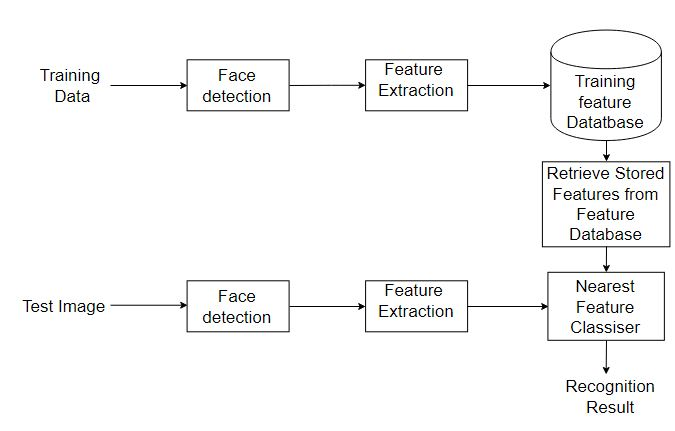
\includegraphics[width = 8cm]{Face_Recognition_Architecture.JPG}
 \caption{ Face Recognition Architecture (Source:\cite{makwana_makwana_2016})}
 \label{fig 1: face recognition architecture}
\end{figure}

Face recognition is an extensively researched subject\cite{zhao2003face} \cite{abate20072d}. Figure \ref{fig 1: face recognition architecture} shows a basic face recognition architecture according to which, every new test image, after undergoing pre-processing, is compared with the training data to recognise the person in the image. Most of the face recognition systems today, perform under unobstructed conditions\cite{phillips2005overview}. In these systems, the faces in the images are directly pointed at the camera. However, in a real world scenario, images seldom contain faces which are unobstructed or  faces that are pointed directly at the camera. Occlusion is defined as the blockage due to an external factor. Occlusion in an image can be due to a number of factors like lighting conditions, glasses, scarves, different poses or even certain facial expressions \cite{wright2009robust}. The human brain excels at recognising faces that could be significantly occluded. Most face recognition systems however, reduce to a chance level accuracy while identifying occluded images. Designing a face recognition system that gives accurate results for images with \MK{\sout{or without}} occlusion is a challenging task due to the missing facial cues from occluded areas of the face. In this project, a comparative study of three widely used face recognition methods has been performed on dataset with and without occlusion condition. The image dataset has been randomly cropped out \MK{to} check the performance of these algorithms on occluded images. The main aim of this project is to understand if existing machine learning methods could be used for face recognition under occluded conditions without compromising on the accuracy. Although, the level of occlusion is not considered,  this project provides a direction for further research into the topic. There are various methods of face recognition such as principal component analysis, independent component analysis, k-nearest neighbour, linear discriminant analysis and convolutional neural networks \cite{zhao2003face}. Out of these methods, principal component analysis, k-nearest neighbour and convolutional neural networks are highly prominent in academia and industry.

\vspace{0.5mm}
By definition, principal component analysis is a mathematical procedure that uses orthogonal transformation to convert a set of values of possibly correlated M face images into a set of K uncorrelated variables called the Eigenfaces
\cite{turk1991face}. Face recognition by PCA is achieved by projecting the test image in the eigenface subspace. Then the distance between the position of test image in eigenspace is compared with the known dataset or the training dataset. Based on this comparison, the person is recognised. k-nearest neighbors is a robust and efficient method used for classification and regression. In this algorithm, the training image data set is separated into multiple classes to predict the classification of a new test image. k-nearest neighbors is one the best face recognition methods as it is a non parametric algorithm. This fact is very helpful as the data typically does not obey the theoretical assumptions. hence prior knowledge of the data is not required for prediction. Neural networks, is another widely preferred face recognition method because of its non linear approach. Convolutional Neural Networks based systems directly learn from the training dataset that is provided and adopt deep learning algorithms to recognise an image. The accuracy of these systems can be significantly improved by appropriate pre-processing and segmentation of the images and by increasing the number of hidden layers \cite{dean2012large}.


There has been a significant amount of research on face recognition systems under unoccluded image conditions. However there has not been enough research on face recognition under occlusion. In this project the methods that have been mentioned above are applied to occluded images. These methods have been chosen as they are state-of-the-art, robust and widely used in the industry and academia. The goal of PCA is to retain only those features that convey the most information\cite{turk1991face}. k Nearest Neighbor algorithm, although is simple in implementation, provides reasonably accurate results\cite{zhang2007ml}. Convolutional neural networks are used for their superior performance and high accuracy\cite{lawrence1997face}.



The remainder of the paper is is structured as follows: Section \ref{sec: 2.Background} provides a brief literature review on face recognition methods. \ref{sec:3 Methodology} describes the methodology followed to implement the algorithms. Section \ref{sec:4 Experimental Setup} gives an overview of the experimental setup to run face recognition algorithms. Section \ref{sec: 5. Results and Analysis} provides a description of the obtained results. Section \ref{sec: 6.Conclusion and Future Work} provides conclusion and future work based on the experiment performed.

\section{Background}
\label{sec: 2.Background}

There are three stages involved in the process of face recognition from an image. They are: (1) face detection (2) feature extraction (3) face recognition. Face detection, as mentioned earlier, is the technology to detect the presence of a human face in an image. Numerous methods can be used to perform face detection and One of the most popular method is to perform face detection is Viola Jones face detector \cite{zafeiriou2015survey}. Although it trains at a slow pace, the advantage of Viola Jones face detector over other methods is swift detection. The key principles involved in face detection using a Viola Jones detector are- the simple haar features, utilization of integral images and several rounds of boosting for feature extraction and selection, and an attentional cascade to only allow windows with faces\cite{zafeiriou2015survey}.

Feature extraction, in simple terms, deals with the removal of all the redundant information from an image, thereby increasing the computation speed and reducing the amount of memory used. Essentially, this stage includes all the pre-processing and normalization of the image. The steps involved are RGB to grayscale transformation, scaling and histogram equalization. Feature extraction is the most complex part of face recognition process. The accuracy of the system is highly dependent on the method used for feature extraction \cite{brunelli1993face}.

Face recognition methods have evolved over time and development of technology. A very simple technique to achieve this is to flatten the test image into a vector, and compute the Euclidean distance between the test image and all the other flattened images from the training dataset. The downside of this technique is that it consumes a large amount of time to compare all images if the dataset is large and is not very accurate. Face recognition methods can largely be classified into appearance-based and model based methods. Appearance based methods are applied to the whole face or particular areas of the face. On the other hand, model based methods are applied to shape and texture of the face. A model of the human face is constructed to detect the facial variations. Since appearance based methods do not use prior knowledge of faces, they fail when images of poor illumination or faces with different poses are tested. Conversely, model based approaches  make use of prior knowledge of faces and hence they are indifferent to any changes in the illumination and pose. However model based systems require a fair amount of time and are complex to implement. Appearance methods are further divided into linear and non linear methods. The most common among linear methods is the principal component analysis. An extension of principal component analysis to perform non linear form of face recognition is kernel principal component analysis. Another widely preferred non linear approach is the neural networks method \cite{agrawal2015evaluation}.

In the recent years, there has been some research into face recognition under partial occlusion. \cite{blanz2003face} introduced a face recognition method which recognises faces irrespective of the pose and light conditions. In accordance with other model based approaches, they simulate a 3D image using graphics from single images. The model is then fitted to the images. Through this model, they account for the variations in pose and illumination. The model is trained from a set of 3D scans of the head. In this paper, they describe the design of the model and the algorithm for fitting it to the images. Finally they provide a framework for face recognition where the faces are represented by 3D shape and texture from the model. 

The methods used to handle face recognition and occlusion can be classified as feature, part and fractal based methods. In part based methods, facial recognition is done by dividing the image into multiple parts. Tan et al. presented a non-metric partial similarity measure to calculate the outstanding similarities between two images and discarding all the unimportant differences between them \cite{tan2006learning}. This will help  extract the intra-personal similarities thereby causing the effect created by occlusions and other variations to be reduced. Kim et al. use two-dimensional principal component analysis for face recognition of occluded images \cite{kim2007occlusion}. Here, a feature matrix is created and the occluded parts of an image are identified by classifying each row of the matrix. The process is divided into two stages- occlusion detection and partial matching. They use a combination of k-NN and 1-NN classifier and similarities between feature matrices on AR face database to develop the face recognition algorithm. The basis of knn algorithm is feature-similarity  i.e. the closeness of the features of any test image to the training images determines the classification of that test image; where Eucledian distance measure is used to find the the distance in the image space \cite{wang2005euclidean}. The distance between test image features and training image feature is calculated and a distance matrix is formed. The distance matrix is summed up and arranged in an increasing order. Based on the value of k, the first k elements are selected and the test image is classified according to the majority class value \cite{zhang2007ml}. Chen et al. suggested the use of kernel principal component analysis algorithm \cite{chen2016recognition}. The images were divided and a certain weight was assigned to each part. The features from each part were then extracted by KPCA to classify and recognise the image.

In fractal based method for handling partial occlusions, the images are partitioned and each region is accessed by iterated function system. The ad hoc measurement of distance using a distance function removes all the unimportant data that is not required for recognition, thereby increasing the speed and accuracy of recognition \cite{abate20072d}.

Feature based methods that are applied to tackle the issue of occlusion take into account the features of an individual like the edges around the eyes and mouth and disregard the other features. Turk et al propose a face recognition method using eigenfaces. Images are represented as a small set of 2D characteristics  \cite{turk1991face}. Principal component analysis gives excellent results in a constrained environment. Here, images under constrained environment indicates that the images are not occluded by any factor. It is a preferred approach as it is simple, fast and has a high learning capability. The eigenvectors of the training dataset define the  feature space. Images are projected onto a feature space to derive unique characteristics. Faces are recognised by comparing the characteristics of the test dataset to the characteristics of the test dataset. The model provided the  capability of near-real-time face recognition. A. M. Martinez takes a probabilistic approach to solve occlusion problem by using an eigenspace representation \cite{martinez2000recognition}. Each image is divided into multiple regions and is analysed to recreate the training set and perform a matching with the images to recognise the face.

Neural networks, is another widely preferred face recognition method because of its non linear approach. Convolutional Neural Networks based systems directly learn from the training dataset that is provided and adopt deep learning algorithms to recognise an image. Using an unaltered convolutional neural network on occluded images, a low level of accuracy will be obtained \cite{chandler2016mitigation}. However, training this network with occluded images improves the accuracy but is still not very efficient in prediction. This can be significantly improved by appropriate pre-processing and segmentation of the images. The flaw with this system is that excessive training will lead to the problem of overfit. Overfit is a situation where the system memorizes all the training data and when new test data with noise is presented, it will not be able to produce an accurate result. There are many libraries available to implement convolutional neural networks\cite{2016arXiv160502688short}\cite{Jia:2014:CCA:2647868.2654889}. TensorFlow\footnote{https://www.tensorflow.org/tutorials} is an open source library for machine learning developed by Google and is based on deep learning DistBelief framework. A convolutional neural network based on TensorFlow is highly robust and has a high accuracy rate even when the faces in the images are occluded.  It offers high flexibility and is relatively simple to use. An advantage of using convolutional neural networks is that some of the pre-processing steps can be skipped \cite{oliveira2017irish}. Keras\footnote{https://keras.io/} is an open source library which runs on top of TensorFlow. Keras makes it easy to build and run convolutional neural networks\cite{chollet2015keras}.

At present, most of the research has been done on face detection and recognition systems of perfectly aligned face images and relatively few studies for images with facial occlusion. Of all the methods that are proposed, most researchers use part based methods in which the image is segmented and then each individual region is analyzed. The most widely implemented face recognition under occlusion techniques are face recognition using principal component analysis, k-nearest neighbours and convolutional neural networks. Each of these methods have been considered on different image datasets. To measure the accuracy of these methods, they should be verified against one dataset. Hence, in this project, all these methods have been implemented on Labelled Faces in the Wild dataset. Furthermore, there is a need to verify the behaviour of these models and find the change in accuracy when regions of the face are occluded in the image.





\section{Methodology}
\label{sec:3 Methodology} 
The following section describes a theoretical analysis of the methods followed to implement the three face recognition systems, i.e. principal component analysis, k-nearest neighbour and convolutional neural networks. The performance of these machine learning algorithms is evaluated by implementing these algorithms on the LFW dataset. The dataset is split into training and test dataset using cross-validation. The system is trained on the training dataset and then evaluated by running test data through it. Subsequently, the test data is randomly occluded and run through the system to compare the difference in accuracies of the prediction among the two datasets. The remainder of this section describes implementation guidelines of the three face recognition methods.


Principal component analysis is a computationally meticulous approach for simplification of data. It aims to convert a set of correlated data into an uncorrelated set called principal components\cite{turk1991face}. Data is split into training and test data using cross validation technique. As the number of features increase, the computation cost and complexity of the system increase which could lead to the problem of overfitting. Instead of indiscriminate elimination of image pixels, principal component analysis is employed to perform dimensionality reduction which can reduce the data from a two dimension plane to a single dimension line. Principal component analysis  attempts to represent the variance in the training data with a reduced number of dimensions. The features are compressed and only the most useful feature combinations are returned. These constitute the eigenfaces. The data is then normalized to make it less redundant. It is performed by rotating into the coordinate space of the principal components. Each dimension is then divided by the standard deviation in that direction to get unit variance and then rotated back. 

Support Vector Machines(SVM) and GridSearchCV have been used to train the model. Support Vector Machines determine a decision boundary such that the distance between two classes of data is maximum. the classifier can easily recognize faces when the data is spread out instead of grouped together. Support Vector Machines are very efficient. however, to further optimize the results the parameters can be altered manually or can be automated using GridSearch module that does a parameter sweep to give the best results.
The general steps to perform face recognition using PCA are:
\begin{enumerate}
\item Train the system using a certain image set.
\item Compute the covariance matrix of the training dataset
\item Extract Eigenfaces using PCA
\item Represent each image with respect to eigenfaces(as a vector of weights)
\item To test the system, calculate the weight of test image. Compare it with the weights already known to the system
\item Recognition is done by matching the weights of the test image to the closest weights that are known to the system. 
\end{enumerate}
	
The model is then tested on an unknown dataset to measure accuracy of recognition. in the next step, data is randomly occluded and used as test dataset. precision, recall, f1-score and support have been calculated along with confusion matrix as a measure of accuracy of prediction. 



k Nearest Neighbour method is preferred over other classifiers due its simplicity and robustness in multi model classification. It also requires lesser execution time and offers better accuracy. It is efficient in classifying test data based on closest training data in the feature space. An image is classified by a taking a majority vote of the neighbouring classes. Euclidean distance measure is most commonly used for this algorithm. The other widely used measures are Manhattan distance, Jaccard distance, Minkowski distance etc. Equation \ref{Equation 1: Euclidean Distance} shows the calculation of Eucldean distance \cite{weinberger2006distance}. 
%%%
%\begin{figure}[h!]
%%\vspace{-0.2cm}
% \centering
% 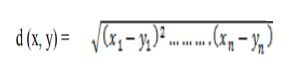
\includegraphics[width = 8cm]{euclidean_distance11.JPG}
% \caption{Euclidean Distance Computation (Source:\cite{weinberger2006distance})}
% \label{fig 4 : Euclidean Distance}
%\end{figure}
%%%
\begin{equation}
\label{Equation 1: Euclidean Distance}
d(x,y) = \sqrt{(x_1-y_1)^2.......(x_n-y_n)}
\end{equation}
Where n is the number of variables, $x_i$ and $y_i$ are the values of the $i^{th}$ variable at points p and q respectively. Using equation \ref{Equation 1: Euclidean Distance}, the euclidean distance between a given test image and each training image features is computed. This forms a distance matrix whose summation value is calculated and sorted in an increasing order. According to the value of k that is specified, the classes are selected and the majority class value determines the classification of the test image \cite{kaur2012k}. k-nearest neighbour algorithm classifies the test images by computing the most common class from the k closest training data points. Each training data point from the k closest classes counts as a vote and the data points is classified as the class with most votes.

The general steps to perform recognition using k-nearest neighbour are:
\begin{enumerate}
\item The training data is divided into respective classes.
\item k closest neighbours to the new test data are found using distance matrix.
\item These points are then analyzed to determine the class of the test data.
\item The class of the test data is determined by majority class value and is assigned to the data.
\end{enumerate}


Convolutional neural networks are made of multiple layers of neurons which can be assigned weights and biases. Input is given to each neuron which performs a dot product. Neural networks are preferred for face recognition methods because of their non linear approach. They are similar to ordinary neural networks in that, they have a loss function on the final layer and use the same mechanism to train the system. Image pixels are given as an input to the network and class scores are obtained as an output. 

%\begin{figure}[h!]
%\vspace{-0.2cm}
 %\centering
 %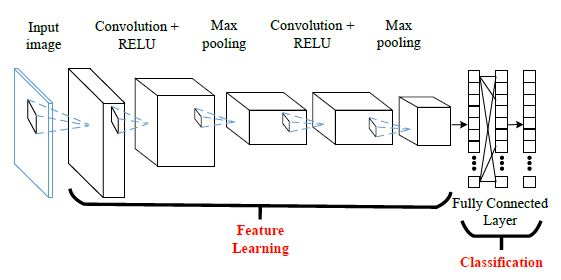
\includegraphics[width = 9cm]{cnn_arch.JPG}
 %\caption{ Convolutional Neural Network (Source:\cite{cheung2012convolutional})}
 %\label{fig 5: Convolutional Neural Network}
%\end{figure}

 The output is another multidimensional array of numbers which serves as an input to the next layer. Every layer of convolutional neural network converts one activation function to another through a differentiable function. As shown in the image, there are three layers used to build a convolutional neural network: Convolution (CONV) Layer, Pooling Layer, and Fully-Connected Layer. 
 
\begin{enumerate}

\item Input layer holds the raw image. The convolution layer computes the dot product.
\item RELU layer is responsible for the activation function.
\item Downsampling operation is performed by the POOL layer.
\item  Fully connected layer is responsible for providing the output with the class scores.

    Keeping with its name, the neurons in this layer are connected to all neurons in the previous layer. Equation \ref{equation 2} shows the convolution operation.


 

\begin{equation}
\label{equation 2}
h_j^{(l)} = \sigma(\Sigma_{i=1}^{n_i} h_i^{(l-1)} * w_{ij}^{(l)} + b_j^{(l-1)}) , l=1,....,L
\end{equation}

where $h^{(l)}_j$ denotes the j-th feature map in the l-th layer, and nl is the number of feature maps in the l-th layer. The network is parameterized by weights $w_{ij}^{(l)}$ and biases $b_j^{(l)}$to be learned\cite{lee2009convolutional}.  Additionally, convolutional layer and fully connected layers perform computations not just using the activation functions from the previous layers but also using their individual weights and biases. But the other layers namely, RELU and POOL, execute a  fixed function. The parameters in the convolutional/fully connected layers are trained using the principle of gradient descent. It is a guided search method. To monitor the error in a model, a separate cost function is used. The aim is to minimise this function to achieve lowest error possible or the maximum accuracy. Gradient descent is a repetitive process of optimization by tweaking certain parameters to find the minimum of a function, i.e. to take small steps that are proportional to the negative of the gradient of the cost at every point. Gradient descent is employed to ensure that the class scores that are output from the network are consistent with the classes in the training image set. Using this underlying principle, CNN transforms raw image pixels to the final class scores. 



\section{Experimental Setup}
\label{sec:4 Experimental Setup} 


This section describes the set of experiments that have been performed to find and analyze the accuracies of the above mentioned face recognition algorithms. To implement these algorithms, scikit learn, TensorFlow, FaceNet \cite{schroff2015facenet} and Keras libraries from Python have been used. Evaluation has been performed by comparing the result of the experiment with occluded and unoccluded images. The basic stages in each of these algorithms are: input stage, processing stage and output. A visualisation of these stages is as shown in figures \ref{fig 2: dataset}, \ref{fig 3:Processing Stage} and \ref{fig 4: Ouput}. The data is split into a training and a test dataset. The systems are trained using LFW dataset and then tested under two conditions. First with unoccluded images from LFW dataset and second by randomly occluding the same images.

\begin{figure}[h!]
%\vspace{-0.2cm}
 \centering
 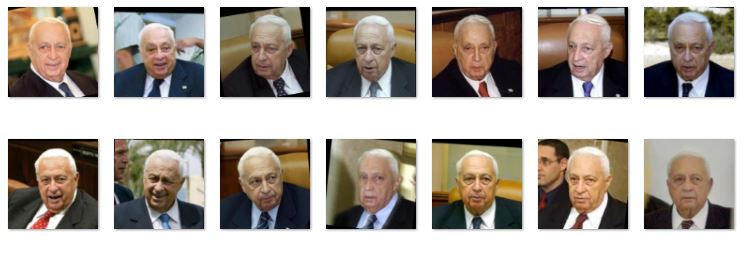
\includegraphics[width = 9cm]{dataset.JPG}
  \caption{ Images from Labeled Faces in the Wild(Source:\cite{LFWTech})}
 \label{fig 2: dataset}
\end{figure}

\begin{figure}[h!]
%\vspace{-0.2cm}
 \centering
 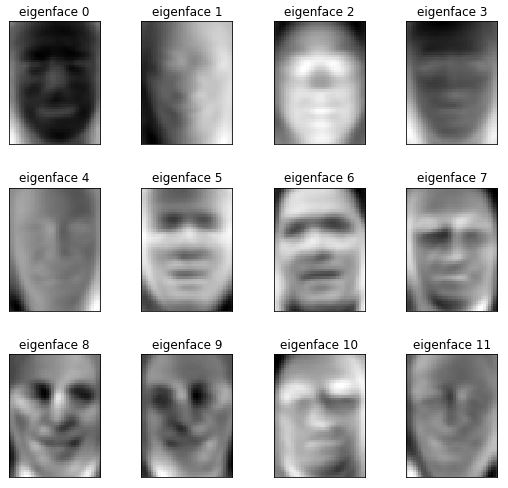
\includegraphics[width = 9cm]{eigenface.JPG}
 \caption{ Images under Processing Stage}
 \label{fig 3:Processing Stage}
\end{figure}

\begin{figure}[h!]
%\vspace{-0.2cm}
 \centering
 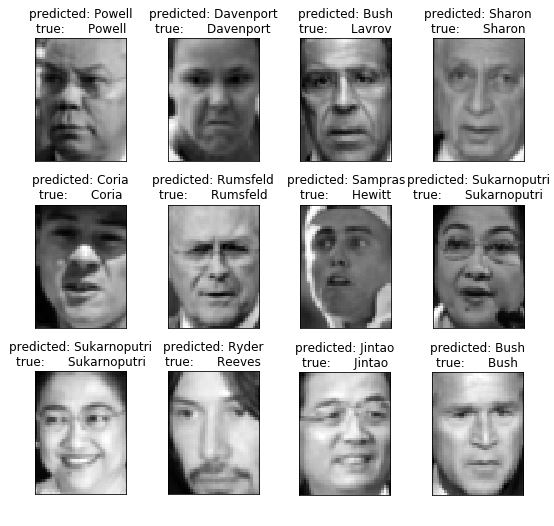
\includegraphics[width = 9cm]{PCA_pred.JPG}
 \caption{Recognised Images}
 \label{fig 4: Ouput}
\end{figure}


\subsection{Data} 
\label{subsec: 4a. Data}
The dataset used for this project is the Labeled Faces in the Wild dataset, a collection of over 13,000 images of celebrities from the internet \cite{LFWTech}. Each face has been labelled and stored under a folder with the name of the person. However, not all people from the dataset have the same number of images. Using the dataset as is, will not yield expected results as any network will not be able to learn and identify a person based on just one image. In order to avoid class imbalance and for the system to train satisfactorily, only few people with most number of images have been selected for this project. Occluded faces are more complicated to recognise than unoccluded ones. To get an occluded image dataset, the images from the training dataset have been randomly cropped out. 

The data is split into training data and test data using stratified k-fold cross validation. Training data is used to train the system while the test set is used to evaluate the performance of the system. Stratification ensures that the test data covers all classes of the training data. In other words, stratification ensures that the test data is a good representation of the training data. It offers a better split in terms of bias and variance than simple cross-validation. 


\subsection{Principal Component Analysis} 
\label{subsec: 4b. Principal Component Analysis}
To implement face recognition using PCA, the LFW image data set is loaded as numpy arrays. PCA function is used to reduce the number of features and extract the eigenfaces. The most significant eigenfaces have been plotted. Support Vector Machines have been used for the classification of the images. Support Vector Machines mark each data point in an n-dimensional spaces according to the number of features that are selected. It gives an optimal hyperplane with maximum margin between classes. Data is categorized based on this hyperplane.


Even though the system is not very complex, it produces efficient results. The algorithm accurately recognises a large number of images from the data. To quantify the efficiency of the algorithm, various measures from sklearn.metrics have been used. The classification report gives the precision, recall, f1-score and support for the classification. 

Precision is the ratio of number true positives to the false positives. Recall is the ratio of number of true positives to the false negatives. While precision shows the capability of the classifier to avoid false positives, recall shows its ability to mark all the positives. the harmonic mean of precision and recall is shown as f1-score. support shows the number of samples in a class that are of true response \cite{scikit-learn}.

\subsection{k-Nearest Neighbour} 
\label{subsec: 4c k-Nearest Neighbour}
k-nearest neighbour algorithm goes through the entire data for every test datapoint to find the k nearest or most similar instances to the training data. scikit-learn library and functions have been used to implement k-nearest neighbour algorithm. The underlying data structure to find the nearest neighbours using Euclidean distance BallTree. It allows to use Minkowski distance to find the nearest neighbours. Minkowski distance with the value of parameter equal to 2 corresponds to Euclidean distance \cite{weinberger2006distance}.

A k-nearest neighbour system is developed. The system is trained on the LFW data. It is trained according to the names of the people in the dataset. The model is saved so that it does not have to train every time a new data is tested. When a new test data is entered, it checks for two closest neighbours to create a distance matrix. These points then determine the name of the person in the image. The majority vote from the two classes is given as the result of this method.
	
\subsection{Convolutional Neural Networks} 
\label{subsec: 4c Convolutional Neural Networks}
One of the major issues for building convolutional neural networks using tensorflow, are the hardware requirements. Since convolutional neural networks are computationally heavy, it is easier to use cloud services to implement them. To execute convolutional neural networks, two approaches have been followed in this project i.e., using fuel library and facenet\cite{schroff2015facenet}. With fuel library, the network was built with three hidden layers that includes two convolutional layers and a single dense layer. Considering this is a very basic neural network, the accuracy achieved was only about 65\%. Hence the second approach had to be followed. The accuracy of a convolutional neural network can be increased by adding more number of hidden layers. The performance of convolutional neural networks also varies according to the weights and bias assigned at each layer. It is a trial and error method to tune the appropriate weights to achieve a high accuracy. This is a major disadvantage of convolutional neural networks. Once the weights are decided, the network trains and performs efficiently. 

FaceNet is a deep convolutional network, with multiple hidden layers, that maps the image data to an Euclidean space. This uses the concept of distance and face similarity i.e. the images of same person with small distances between them will be grouped together. Further, there will be a significant difference between images of different people. Subsequently, the recognition task can be completed using k-nearest neighbour algorithm. The system uses a triplet image set for training. The triplet is chosen such that two of the images match and one does not. Therefore, the images that match will have smaller distance and can be grouped together while the images that do not match have a larger distance between them \cite{schroff2015facenet}. The model represents each the faces in the training set into a 128 dimensional vector which are labeled and used for recognition of faces. When a new test image is entered into the system, it goes through the network to form a 128 dimensional vector. This vector is then compared with the training set. The lowest distance between the test image and training set is used to recognise the face in the image. 

After the implementation of these methods, the next step was to test their performance over a test data. As mentioned earlier, the data was split into training and test data. These methods were run on the test dataset and the accuracy was noted. Subsequently, the test dataset was occluded by randomly cropping a portion of the images. The above mentioned methods were then run on occluded data to check their accuracy of face recognition.

\section{Analysis and Results}
\label{sec: 5. Results and Analysis}
In this section, the results obtained from the experiments have been presented. Table \ref{table 1} shows the accuracy of face recognition for each of the methods. These results vary with a margin of 3\%. For each method, the system was trained on unaltered LFW data. Each system was then tested under both unoccluded and occluded conditions. From the table \ref{table 1} it follows that, with 88\% and 99\% principal component analysis and convolutional neural networks show a high accuracy in recognising faces from unoccluded images. Among these methods, k-Nearest neighbours gives the least accuracy of only 82.3\%. However, the performance of principal component analysis substantially decreases by more than 15\% when it is applied to occluded images. Even though k-nearest neighbour method shows low accuracy over unoccluded images, it shows a smaller change of about 10\% in accuracy over occluded images when compared to principal component analysis. In comparison with the other two methods convolutional neural networks show a very high accuracy of about 99\% and 97\% under unoccluded and occluded conditions respectively. Further, there is a comparatively smaller difference of only about 3\% in the accuracy of face recognition over images with and without occlusion.

\begin{table}[h]
\centering
\caption{Overall Face Recognition Accuracy of Different Methods}
\label{table 1}
\begin{tabular}{|c|c|c|c|}
\hline
\textbf{Methods} & \begin{tabular}[c]{@{}c@{}}Principal Component \\ Analysis\end{tabular} & \begin{tabular}[c]{@{}c@{}}k Nearest\\  Neighbours\end{tabular} & \begin{tabular}[c]{@{}c@{}}Convolutional\\ Neural \\ Networks\end{tabular} \\ \hline
\textbf{\begin{tabular}[c]{@{}c@{}}Accuracy\\ (Unoccluded \\ Images)\end{tabular}} & 88.1\% & 82.3\% & 99\% \\ \hline
\textbf{\begin{tabular}[c]{@{}c@{}}Accuracy\\ (Occluded\\  Images)\end{tabular}} & 73.5\% & 71.9\% & 97.4\% \\ \hline
\end{tabular}
\end{table}

From the results, it shows that convolutional neural networks have the highest accuracy and show little difference in comparison with the accuracies given by principal component analysis and k nearest neighbour methods. The accuracy of pre

\section{Conclusion and Future Work}
\label{sec: 6.Conclusion and Future Work}

In this project, a comparative analysis of three widely used face recognition methods: Principal Component Analysis, k-Nearest Neighbour and Convolutional Neural Networks has been presented with the help of an experiment. The systems are trained on LFW data. They are then tested on a test dataset and again by occluding the dataset. From the experiment, it shows that Among the three methods that were chosen, convolutional neural networks have shown to be most accurate. Convolutional neural networks are advantageous over other systems due to minimal preprocessing and domain knowledge required to run them. They can effectively handle large amounts of data without any deterioration in performance. Despite their high accuracy rates, Convolutional neural networks have certain drawbacks. The time required to train these networks increases with the amount of data and number of layers. It also requires high computation power, processing speed and memory. As shown, each algorithm has its own benefits and drawbacks. Since principal component analysis uses only the dominant feature, the time required for computation is low. It offers a simple and straightforward method for feature extraction and gives consistent results. k-nearest neighbour exhibits robust performance and is particularly beneficial due to its non-parametric approach. A meaningful ranking of these methods depends on a number of factors like the level of occlusion, other methods under consideration, the amount of data used for training and other generic factors need to be considered. Appropriate algorithm should be used for specific applications. 

This project shows the superior accuracy offered by convolutional neural networks under the conditions that the data is occluded by cropping the images, only above mentioned three methods are considered and training is done on unoccluded images. This project provides the following directions for future work, 
\begin{enumerate}
\item Analysis of methods by varying the level of occlusion of the images. This can help to find a threshold of occlusion that can be applied to images beyond which the above described face recognition methods resort to only a chance level accuracy. In such cases, new algorithms need to be developed which can easily identify occluded images.

\item Occluded images can be used for training which could affect the accuracy of the system.

\item The area of occlusion in an image can be varied to get further insight into the behaviour of face recognition methods. 
Most of the work deals with face recognition using two dimensional images.

\item The accuracy of prediction can be enhanced by using three dimensional face recognition systems.

\item The creation of occlusion can be automated to test the methods more effectively.


\end{enumerate}
 


\section*{Acknowledgment}
This work was supported by Dublin City University (DCU), Dublin, Ireland and Dr.Alessandra Mileo, School of Computing, DCU.

\bibliographystyle{IEEEtran}
\bibliography{refs.bib}

\end{document}
